\part{Analytical mechanics}
\chapter{Introduction}
\section{One particle systems}
\subsection{Definitions}
For a single particle system of mass \textit{m}, which is moving along a trajectory we can define some properties:
\begin{itemize}
    \item Position: $\vec{r}$
    \item Velocity: $\vec{v} = \dfrac{\mathrm{d} \vec{r}}{\mathrm{d} t}=\dot{\vec{r}}$, which magnitude is called \textit{speed}
    \item Acceleration: $\vec{a}=\dfrac{\mathrm{d}^2 \vec{r}}{\mathrm{d} t^2}=\dot{\vec{v}}=\ddot{\vec{r}}$
\end{itemize}
\begin{figure}[H]
    \centering
    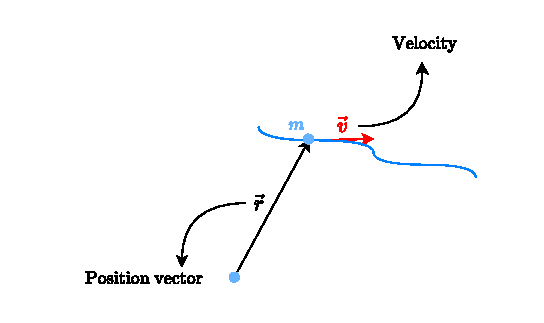
\includegraphics[width=0.6\textwidth]{res/svg/onepartsys.drawio}
    \caption{One particle system}
    \label{fig:image1}
\end{figure}

From that we can derive some quantities:
\begin{itemize}
    \item Linear momentum: \begin{equation}\vec{p}=m\vec{v}\end{equation} While $m$ is constant
    \item Total force applied: \begin{equation}\vec{F}=\dot{\vec{p}}=\dfrac{\mathrm{d} \vec{p}}{\mathrm{d} t}=m\vec{a}\end{equation}The first equality is the original formulation for Newton's second law.\\From this follows the conservation of linear momentum:
    \begin{equation}\vec{F}=0 \iff\dot{\vec{p}}=0 \iff\vec{p}\;\mathrm{is\;constant} \iff\vec{v}\;\mathrm{is\;constant}\end{equation}
    \item Angular momentum:
    \begin{equation}
        \vec{L_{\Omega}} = \left(\vec{r}-\vec{r}_{\Omega}\right) \cross m\vec{v} = \left(\vec{r}-\vec{r}_{\Omega}\right) \cross \vec{p}
    \end{equation}
    The angular momentum is a pseudo-vector and it is always calculated with reference to a generic point $\Omega$.
    \begin{figure}[H]
        \centering
        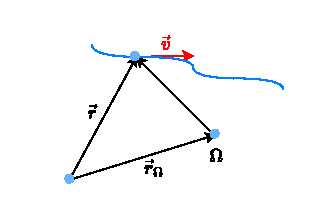
\includegraphics[width=0.6\textwidth]{res/svg/omegareference.drawio}
        \caption{Reference point for angular momentum}
        \label{fig:image2}
    \end{figure}
    Trying to differentiate the angular momentum we get:
    \begin{equation}
      \begin{split}
        \dfrac{\mathrm{d}\vec{L}_{\Omega}}{\mathrm{d}t} &= \dfrac{\mathrm{d}}{\mathrm{d}t}\left(\left(\vec{r}-\vec{r}_{\Omega}\right) \cross \vec{p}\right) = \dot{\vec{r}}\cross\vec{p} - \dot{\vec{r}}_{\Omega}\cross\vec{p} + \left(\vec{r}-\vec{r}_{\Omega}\right) \cross \vec{F} = \\[8pt]
        &= - \vec{v}_{\Omega}\cross\vec{p} + \vec{\tau}_{\Omega}
      \end{split}
    \end{equation}
    If $\Omega$ is at rest we can choose $\Omega = O$ which implies:
    \begin{equation}
        \dfrac{\mathrm{d}\vec{L}_{\Omega}}{\mathrm{d}t} = \vec{\tau}_{\Omega}
    \end{equation}
    From which follows the conservation of angular momentum:
    \begin{equation}
        \vec{\tau}_{\Omega} = 0 \iff\vec{L}_{\Omega}\;\mathrm{is\;constant}
    \end{equation}
    If $\vec{L}_{\Omega}$ is fixed then the trajectory happens on a plane.
    \begin{figure}[H]
        \centering
        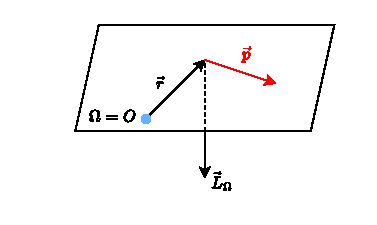
\includegraphics[width=0.6\textwidth]{res/svg/singleplanemotion.drawio}
        \caption{Motion on a single plane}
        \label{fig:image3}
    \end{figure}
\end{itemize}
\subsection{Work}
The work done by the total force on a particle from point $P_1$ to $P_2$ along a generic path can be visualized as:
\begin{figure}[H]
    \centering
    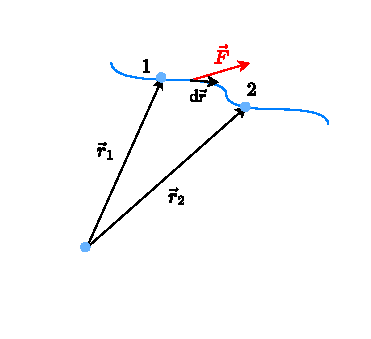
\includegraphics[width=0.5\textwidth]{res/svg/work.drawio}
    \caption{Work of the total force}
    \label{fig:image4}
\end{figure}
and is evaluated as:
\begin{equation} \label{e:total_work}
  \begin{split}
    W_{12} &= \int_{P_1}^{P_2}\vec{F}\cdot\mathrm{d}\vec{r} = \int_{P_1}^{P_2}\dfrac{\mathrm{d}}{\mathrm{d}t}(m\vec{v})\cdot\mathrm{d}\vec{r} = \int_{P_1}^{P_2}\dfrac{\mathrm{d}}{\mathrm{d}t}(m\vec{v})\cdot\vec{v}\mathrm{d}t = \\[8pt]
    &= m\int_{P_1}^{P_2}\vec{v}\mathrm{d}v = \dfrac{1}{2}mv^2\bigg|_{P_1}^{P_2} = \dfrac{1}{2}mv_2^2 - \dfrac{1}{2}mv_1^2 = T_2 -T_1\\[8pt]
    &\boxed{W_{12} = T_2 -T_1}
  \end{split}
\end{equation}
So the work done by the total force is the difference of the kinetic energy $T$ from point $P_1$ to $P_2$.\\
A force $\vec{f}$ is \textbf{conservative} if its work does not depend on the path:
\begin{equation}
    W_{12} = \int_{P_1,\gamma_1}^{P_2}\vec{f}\cdot\mathrm{d}\vec{r} = \int_{P_1,\gamma_2}^{P_2}\vec{f}\cdot\mathrm{d}\vec{r}\;\;\forall\;\gamma_1, \gamma_2
\end{equation}
\[\Updownarrow \]
\begin{equation}
  \begin{split}
    \int_{P_1,\gamma_1}^{P_2}\vec{f}\cdot\mathrm{d}\vec{r} - \int_{P_1,\gamma_2}^{P_2}\vec{f}\cdot\mathrm{d}\vec{r} &= 0 \\[8pt]
    \int_{P_1,\gamma_1}^{P_2}\vec{f}\cdot\mathrm{d}\vec{r} + \int_{P_2,\gamma_2}^{P_1}\vec{f}\cdot\mathrm{d}\vec{r} &= 0 \\[8pt]
    \oint\vec{f}\cdot\mathrm{d}\vec{r} &= 0
  \end{split}
\end{equation}
So if a force is conservative then its circulation is always 0 for any closed path.\\
Also if $\vec{f}$ is conservative we can find a scalar function such that:
\begin{equation}
    \int_{P_1,\gamma}^{P_2}\vec{f}\cdot\mathrm{d}\vec{r} = V_1-V_2
\end{equation}
This function is called the \textbf{potential}:
\begin{equation}
    V_1-V_2 = \int_{P_1}^{P_2}(-\mathrm{d}V) \Rightarrow \vec{f}\cdot\mathrm{d}\vec{r} = -\mathrm{d}V = -\grad V \cdot \mathrm{d}\vec{r}
\end{equation}
\begin{equation}
    \vec{f} = -\grad V
\end{equation}
If the total force $\vec{F}$ is conservative (sum of conservative forces) then:
\begin{equation}
    \vec{F} = \bigsum_{i=1}^{N} \vec{f}_i
\end{equation}
\begin{equation}
    W_{12}=\int_{P_1}^{P_2}\vec{f}\cdot\mathrm{d}\vec{r} = \int_{P_1,\gamma}^{P_2}-\grad V\cdot\mathrm{d}\vec{r}
\end{equation}
Where $V$ is the sum of the potential of the single forces. Now from \eqref{e:total_work}, for conservative forces we get:
\begin{equation} \label{e:mech_energy}
    T_2 - T_1 = V_1 - V_2 \iff T_1 + V_1 = T_2 + V_2\iff E_1 = E_2
\end{equation}
Where $E$ is the total \textbf{mechanical energy} of the system.\\
There can be cases such that:
\begin{equation}
    \vec{F} = -\grad V \;\;\;\mathrm{but}\;V=V(\vec{r},t)
\end{equation}
then $\vec{F}$ cannot be conservative. We can show this by computing $\mathrm{d}V$:
\begin{equation}
    \begin{split}
      -\mathrm{d}V &= -\left(\dfrac{\partial V}{\partial x}\mathrm{d}x + \dfrac{\partial V}{\partial y}\mathrm{d}y + \dfrac{\partial V}{\partial z}\mathrm{d}z + \dfrac{\partial V}{\partial t}\mathrm{d}t\right) = \\[8pt]
    &= -\grad V \cdot\mathrm{d}\vec{r} - \dfrac{\partial V}{\partial t}\mathrm{d}t \neq \vec{F}\cdot\mathrm{d}\vec{r} \Rightarrow \int_{P_1}^{P_2}\vec{F}\cdot\mathrm{d}\vec{r} \neq V_1-V_2
    \end{split}
\end{equation}
\section{Multiple particles systems}
\subsection{Definitions}
Similarly to what we established for one particle systems we can define some main characteristics for multiple particles systems:
\begin{itemize}
    \item Mass:\begin{equation}
        M = \bigsum_{i=1}^{N} m_i
    \end{equation}
    \item Linear momentum:\begin{equation}
        \vec{P} = \bigsum_{i=1}^{N} \vec{p}_i
    \end{equation}
    \item Angular momentum (with respect to $\Omega$):\begin{equation}
        \vec{L}_{\Omega} = \bigsum_{i=1}^{N} \left(\left(\vec{r}_i-\vec{r}_{\Omega}\right) \cross \vec{p}_i\right)
    \end{equation}
    \item Average position (centre of mass): \begin{equation} \label{e:centre_of_mass}
        \vec{R} = \dfrac{\bigsum_{i=1}^{N}m_i\vec{r}_i}{\bigsum_{i=1}^{N}m_i}
    \end{equation}
    From this trivially follows:
    \begin{equation}
        \begin{split}
          M \vec{R} &= \bigsum_{i=1}^{N}m_i\vec{r}_i \\[8pt]
          \dfrac{\mathrm{d}}{\mathrm{d}t}(M \vec{R}) &= \dfrac{\mathrm{d}}{\mathrm{d}t}\left(\bigsum_{i=1}^{N}m_i\vec{r}_i\right) \\[8pt]
          M \dot{\vec{R}} &= \vec{P}
        \end{split}
    \end{equation}
    Where $\vec{v}_{CM} = \dot{\vec{R}}$ is the velocity of the centre of mass.
\end{itemize}
\subsection{Newton's third law}
The total force on a single particle contains two components:
\begin{itemize}
    \item internal forces
    \item external forces
\end{itemize}
\begin{equation}
    \vec{F}_i = \vec{F}_i^{(\mathrm{ext})} + \bigsum_{i\neq j}^{N}\vec{F}_{ji}
\end{equation}
We will restrict to the case where $\vec{F}_{ji} = -\vec{F}_{ij}$. This is called \textbf{weak action law}, since it only requires that the forces are equal and opposite, but it is not necessary that they both lie on the same line.\\
\textbf{Newton's third law} (strong action law) is not always true. Let's show a counterexample.\\
Let there be two charges $q_1,q_2$ with velocity $v_1,v_2$ such that $v_1\perp v_2$. Analysing the moment when particle 2 is on the same line of motion of particle 1, for electrostatic forces we get:
\[\norm{\vec{r}_{12}} = \norm{\vec{r}_{21}} = r\]
\[\vec{r}_{12} = - \vec{r}_{21}\]
\begin{equation}
    \vec{F}_{12} = k\dfrac{q_1q_2}{r^2}\hat{u}_{12} = k\dfrac{q_1q_2 \vec{r}_{12}}{r^3}
\end{equation}
\begin{equation}
    \vec{F}_{21} = k\dfrac{q_1q_2}{r^2}\hat{u}_{21} = k\dfrac{q_1q_2 \vec{r}_{21}}{r^3}
\end{equation}
So these forces satisfy both action laws, but these are not the only forces on the charges. Let's analyse the Lorentz's forces. Particle 1 feels a magnetic field:
\begin{equation}
    \vec{B}_{21} = \dfrac{\muz}{4\pi}\dfrac{q_2\vec{v}_2\cross\vec{r}_{21}}{r} \neq 0
\end{equation}
Instead particle 2 does not feel any magnetic field since in the chosen moment it is in the direction of motion of the other charge so we have:
\begin{equation}
    \vec{B}_{12} = \dfrac{\muz}{4\pi}\dfrac{q_1\vec{v}_1\cross\vec{r}_{12}}{r} = 0
\end{equation}
This means that the Lorentz's forces are:
\begin{equation}
    \vec{F}_{21} = q_1\vec{v}_1\cross\vec{B}_{21} \neq 0
\end{equation}
\begin{equation}
    \vec{F}_{12} = q_2\vec{v}_2\cross\vec{B}_{12} = 0
\end{equation}
Hence $\vec{F}_{21} \neq \vec{F}_{12}$ and Newton's thrid law is not satisfied.\\
Since we restrict our cases we have:
\begin{equation}
    \begin{split}
      \vec{F} &= \bigsum_{i=1}\vec{F}_i = \bigsum_{i=1}\vec{F}_i^{\;(ext)} + \cancel{\bigsum_{i=1}\bigsum_{j\neq i}\vec{F}_i} \\[8pt]
      \vec{F} &= \bigsum_{i=1}\vec{F}_i = \bigsum_{i=1}\dfrac{\dd{\vec{p}_i}}{\dd{t}} = \dfrac{\dd{}}{\dd{t}}\bigsum_{i=1}\vec{p}_i = \dfrac{\dd{\vec{P}}}{\dd{t}}
    \end{split}
\end{equation}
But also:
\begin{equation}
    \dfrac{\dd{\vec{P}}}{\dd{t}} = \bigsum_{i=1}\vec{F}_i^{\;(ext)}
\end{equation}
So (only if weak action law holds):
\begin{equation}
    \vec{F} = \dfrac{\dd{\vec{P}}}{\dd{t}}
\end{equation}
\subsection{Angular momentum}
Starting from the definition:
\begin{equation}
    \vec{L}_{\Omega} = \bigsum_{i}\brackets{\vec{r}_i-\vec{r}_{\Omega}}\cross\vec{p}_i
\end{equation}
\begin{equation}
    \begin{split}
      \dfrac{\dd{\vec{L}_{\Omega}}}{\dd{t}} &= \bigsum_{i}\dfrac{\dd{}}{\dd{t}}\brackets{\vec{r}_i-\vec{r}_{\Omega}}\cross\vec{p}_i + \bigsum_{i}\brackets{\vec{r}_i-\vec{r}_{\Omega}}\cross\dfrac{\dd{\vec{p}_i}}{\dd{t}} = \\[8pt]
      &= \cancel{\bigsum_{i}\vec{v}_i\cross\vec{p}_i}-\bigsum_{i}\vec{v}_{\Omega}\cross\vec{p}_i + \bigsum_{i}\brackets{\vec{r}_i-\vec{r}_{\Omega}}\cross\vec{F}_i = \\[8pt]
      &= -\vec{v}_{\Omega}\cross\bigsum_{i}\vec{p}_i + \bigsum_{i}\brackets{\vec{r}_i-\vec{r}_{\Omega}}\cross\vec{F}_i = -\vec{v}_{\Omega}\cross\vec{P} + \bigsum_{i}\brackets{\vec{r}_i-\vec{r}_{\Omega}}\cross\vec{F}_i
    \end{split}
\end{equation}
We can simplify the first term since $\vec{v}_i \parallel \vec{p}_i$ and we can also see that the last term is the \textbf{total torque} $\vec{\tau}_{\Omega}$, which is the result of both the internal and external forces.
\begin{equation} \label{e:first_angular_expression}
    \dfrac{\dd{\vec{L}_{\Omega}}}{\dd{t}} = -\vec{v}_{\Omega}\cross\vec{P} + \vec{\tau}_{\Omega}
\end{equation}
If we restrict to the strong action law we get:
\begin{equation}
    \begin{split}
      \vec{\tau}_{\Omega} &= \bigsum_{i}\brackets{\vec{r}_i-\vec{r}_{\Omega}}\cross\vec{F}_i = \bigsum_{i}\brackets{\vec{r}_i-\vec{r}_{\Omega}}\cross\brackets{\vec{F}_i^{\;(ext)}+ \bigsum_{i\neq j}\vec{F}_{ji}} = \\[8pt]
    &= \bigsum_{i}\brackets{\vec{r}_i-\vec{r}_{\Omega}}\cross\vec{F}_i^{\;(ext)} + \cancel{\bigsum_{i}\brackets{\brackets{\vec{r}_i-\vec{r}_{\Omega}}\cross\bigsum_{i\neq j}\vec{F}_{ji}}} = \vec{\tau}^{\;(ext)}
    \end{split}
\end{equation}
We can cross out the second term since the sum only has terms such as:
\begin{equation}
    \vec{r}_i\cross\vec{F}_{ji} + \vec{r}_j\cross\vec{F}_{ij}- \cancel{{\vec{r}_{\Omega}\cross\vec{F}_{ij}+\vec{r}_{\Omega}\cross\vec{F}_{ji}}}
\end{equation}
This first simplification is a trivial consequence of weak action law. In order to simplify the other term we can realize that if strong action law holds then both $\vec{F}_{ij}$ and $\vec{F}_{ji}$ lie on the line of $\vec{r}_i-\vec{r}_j$ and have opposite directions.
So we get:
\begin{equation}
    \bigsum_{i}\brackets{\brackets{\vec{r}_i-\vec{r}_{\Omega}}\cross\bigsum_{i\neq j}\vec{F}_{ji}} = 0
\end{equation}
Going back to \eqref{e:first_angular_expression} we get:
\begin{equation}
    \dfrac{\dd{\vec{L}_{\Omega}}}{\dd{t}} = -\vec{v}_{\Omega}\cross\vec{P} + \vec{\tau}^{\;(ext)}
\end{equation}
The first term can be 0 if:
\begin{itemize}
    \item $\Omega$ is at rest
    \item $\Omega$ is a point such that $\vec{v}_{\Omega} \parallel \vec{P}$ (for example the centre of mass)
    \item $\vec{P}=0$
\end{itemize}
So in the case of $\Omega = \mathrm{CM}$ we have:
\begin{equation} \label{e:first_cardinal}
    \dfrac{\dd{\vec{L}_{\Omega}}}{\dd{t}} = \vec{\tau}_{\Omega}
\end{equation}
Then:
\begin{equation}
    \vec{L}_{\Omega}\;\mathrm{is\;constant} \iff \vec{\tau}_{\Omega}^{\;(ext)}=0
\end{equation}
The centre of mass also satisfies:
\begin{equation}
    \vec{P} = M\dvec{R}
\end{equation}
as if the mass was all concentrated in the CM. But for angular momentum:
\begin{equation}
    \vec{L}_{\Omega} \neq (\vec{R}-\vec{r}_{\Omega})\cross\vec{P}
\end{equation}
instead this is true:
\begin{equation}
    \vec{L}_{\Omega} = (\vec{R}-\vec{r}_{\Omega})\cross\vec{P} + \vec{L}'_{CM}
\end{equation}
Where $\vec{L}'_{CM}$ is the total angular momentum evaluated in the frame of reference of the centre of mass.\\
From this we can state \textbf{Konig's theorem}:
\begin{equation}
    T = \dfrac{1}{2}\bigsum_i m_i v_i^2 = T_{CM} + T' = \dfrac{1}{2}M v_{CM}^2 + T'
\end{equation}
Where $T'$ is the kinetic energy associated to the motion with respect to the centre of mass.\\
Now we can analyse the work of the system of particles:
\begin{equation}
    \begin{split}
      W_{12} &= \bigsum_i\int_{1}^{2}\vec{F}_i = \int_{1}^{2}\bigsum_i\vec{F}_i = \int_{1}^{2}\bigsum_i\brackets{\vec{F}_i^{\;(ext)} + \bigsum_{j\neq i}\vec{F}_{ji}}\cdot \dd{\vec{r}_i} = \\[8pt]
    &= \int_{1}^{2}\brackets{\bigsum_i\vec{F}_i^{\;(ext)} + \bigsum_i\bigsum_{j\neq i}\vec{F}_{ji}}\cdot \dd{\vec{r}_i}
    \end{split}
\end{equation}
The term $\bigsum_i\bigsum_{j\neq i}\vec{F}_{ji}\cdot \dd{\vec{r}_i}$ is not necessarily 0, but it is 0 in the case of rigid bodies.\\
If external forces are conservative:
\begin{equation}
    \vec{F}_i^{\;(ext)} = -\grad_i V_i
\end{equation}
The gradient with respect to i is $\grad_i = \brackets{\partial_{x_i}, \partial_{y_i}, \partial_{z_i}}$. So the work of external forces is just:
\begin{equation}
    \begin{split}
      W_{12}^{\;(ext)} &= \int_{1}^{2}\bigsum_i\brackets{\vec{F}_i\cdot\dd{\vec{r}_i}} = -\bigsum_i\int_{1}^{2}\grad_i V_i\cdot\dd{\vec{r}_i} =\\[8pt]
    &= -\bigsum_i\int_{1}^{2}\dd{V_i} = -\bigsum_i V_i\bigg|_1^2
    \end{split}
\end{equation}
Now defining $V^{\;(ext)} = \bigsum_i V_i$ we get:
\begin{equation}
    W_{12}^{\;(ext)} = V^{\;(ext)}_1 - V^{\;(ext)}_2
\end{equation}
Now we can see that if forces obey both the strong and the weak action law both $\vec{F}_{ji}$ and $\vec{F}_{ij}$ lie on the line of $\vec{r}_{ij} = \vec{r}_i-\vec{r}_j$ as shown in this example:
\begin{figure}[H]
    \centering
    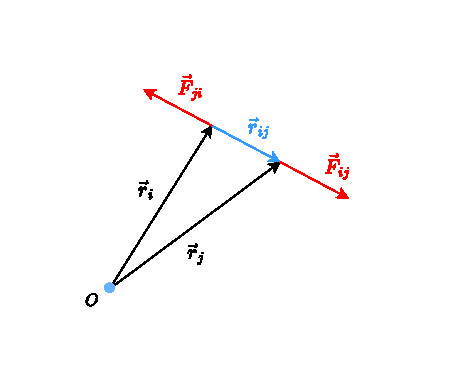
\includegraphics[width=0.5\textwidth]{res/svg/forcesstronglaw.drawio}
    \caption{Forces with strong action law}
    \label{fig:image5}
\end{figure}
Now assuming the forces are conservative we can express them as:
\begin{itemize}
    \item $\vec{F}_{ij}= -\grad_{j}V_{ij}$
    \item $\vec{F}_{ji}= -\grad_{i}V_{ji}$
\end{itemize}
But in this case $V_{ij}=V_{ji}$ so, from the strong action law we get:
\begin{equation}
    -\grad_iV_{ij}=\grad_jV_{ij}
\end{equation}
We can also express both forces with a unique gradient:
\begin{equation}
    \grad_{ij} = \brackets{\dfrac{\partial}{\partial(x_j-x_i)},\dfrac{\partial}{\partial(y_j-y_i)},\dfrac{\partial}{\partial(z_j-z_i)}}
\end{equation}
For the first force we have:
\begin{equation}
    \begin{split}
      \vec{F}_{ji} &= -\grad_iV_{ij}=-\brackets{\dfrac{\partial V_i}{\partial x_i },\dfrac{\partial V_i}{\partial y_i },\dfrac{\partial V_i}{\partial z_i }} = \\[8pt]
      &=-\brackets{\dfrac{\partial V_i}{\partial x_i}\dfrac{\partial r_{ij}}{\partial r_{ij}},\dfrac{\partial V_i}{\partial y_i }\dfrac{\partial r_{ij}}{\partial r_{ij}},\dfrac{\partial V_i}{\partial z_i }\dfrac{\partial r_{ij}}{\partial r_{ij}}}
    \end{split}
\end{equation}
The partial derivatives of $r_{ij}$ are in the form of:
\begin{equation}
    \begin{split}
      \dfrac{\partial r_{ij}}{\partial x_i} &= \dfrac{\partial }{\partial x_i}\sqrt{(x_j-x_i)^2 + (y_j-y_i)^2+ (z_j-z_i)^2} = \\[8pt]
      &= \dfrac{(x_j-x_i)}{\sqrt{(x_j-x_i)^2 + (y_j-y_i)^2+ (z_j-z_i)^2}}
    \end{split}
\end{equation}
So the sum becomes:
\begin{equation}
    \dfrac{(x_j-x_i)+(y_j-y_i)+(z_j-z_i)}{\sqrt{(x_j-x_i)^2 + (y_j-y_i)^2+ (z_j-z_i)^2}} = \dfrac{\vec{r}_{ij}}{\norm{\vec{r}_{ij}}} = \hat{u}_{ij}
\end{equation}
And so we get that the force is:
\begin{equation}
    \vec{F}_{ji}= \dfrac{\partial V}{\partial r_{ij}}\hat{u}_{ij} = \grad_{ij}V
\end{equation}
Doing the same for $\vec{F}_{ij}$ we get:
\begin{equation}
    \vec{F}_{ij}= -\dfrac{\partial V}{\partial r_{ij}}\hat{u}_{ij}= -\grad_{ij}V
\end{equation}
If the internal forces are conservative $V$ must depend only on the magnitude of the distance ($r_{ij}$). Hence:
\begin{equation}
    W^{(int)}=\dfrac{1}{2}\int_{1}^{2}\bigsum_i\bigsum_j\vec{F}_{ji}\cdot\dd{\vec{r}_i}
\end{equation}
The double summation contains terms such as:
\begin{equation}
    \vec{F}_{ji}\cdot\dd{\vec{r}_i} + \vec{F}_{ij}\cdot\dd{\vec{r}_j} = \grad_{ij}V\cdot\dd{\vec{r}_i} + -\grad_{ij}V\cdot\dd{\vec{r}_j} = -\grad_{ij}V\cdot\brackets{\dd{\vec{r}_i}-\dd{\vec{r}_j}}
\end{equation}
Now naming the differential $\dd{\vec{r}_{ij}}=\dd{\vec{r}_i}-\dd{\vec{r}_j}$ and recalling that $-\grad_{ij}V\cdot\dd{\vec{r}_{ij}} = -\dd{V_{ij}}$ we get:
\begin{equation}
    W^{(int)}=-\dfrac{1}{2}\int_{1}^{2}\bigsum_i\bigsum_j\dd{V_{ij}} = -\dfrac{1}{2}\bigsum_i\bigsum_j V_{ij}\bigg|_{1}^{2}
\end{equation}
So the total work is:
\begin{equation}
    W = W^{\;(ext)}+W^{(int)}= -\bigsum_i V_i\bigg|_{1}^{2} -\dfrac{1}{2}\bigsum_i\bigsum_j V_{ij}\bigg|_{1}^{2}
\end{equation}
Defining $V=-\bigsum_i V_i -\dfrac{1}{2}\bigsum_i\bigsum_j V_{ij}$ the total work is:
\begin{equation}
    W = V_1-V_2
\end{equation}
But the total work is also:
\begin{equation}
    W = \int_{1}^{2}\bigsum_i \vec{F}_i \cdot \dd{r_i}= \bigsum_i \int_{1}^{2} \vec{F}_i \cdot \dd{r_i} = T_2 - T_1
\end{equation}
So, for conservative systems we get:
\begin{equation}
    T_2 - T_1 = V_1 - V_2 \iff T_2 + V_2 = T_1 + V_1 \iff E_2 = E_1
\end{equation}
Which is the mathematical expression for the conservation of mechanical energy.
